\documentclass[czech]{beamer}
\usepackage{babel}
\usepackage{svg}
\usepackage{subfig}
\usepackage{siunitx}

\sisetup{
  per-mode=symbol,
}

\renewcommand{\thesubfigure}{\relax}  % Do nothing for the counter »subfigure«

\DeclareSIUnit\hold{chyt}

\usepackage{fontawesome5}

\hypersetup{
  colorlinks,
  allcolors=.,
  urlcolor=blue,
}

% use the focus theme (without fira)
\usetheme[nofirafonts]{focus}
\usefonttheme{serif}

% shamelessly stolen from https://www.patrickbaylis.com/posts/2018-10-11-beamer-resizing/
\usepackage{adjustbox}
\makeatletter
\newcommand{\fitimage}[2][\@nil]{
	\begin{figure}
		\begin{adjustbox}{width=0.9\textwidth, totalheight=\textheight-2\baselineskip-2\baselineskip,keepaspectratio}
			\includegraphics{#2}
		\end{adjustbox}
		\def\tmp{#1}%
	 \ifx\tmp\@nnil
			\else
			\caption*{#1}
		\fi
	\end{figure}
}
\makeatother

\setlength{\belowcaptionskip}{-7pt}

% bullets
\setbeamertemplate{itemize item}{$\bullet$}
\setbeamertemplate{itemize subitem}{$\bullet$}
\setbeamertemplate{itemize subsubitem}{$\bullet$}
\setbeamercolor{itemize subsubitem}{fg=main}

% code
\usepackage{minted}
\setminted[python]{
	linenos,
	mathescape=true,
	escapeinside=||,
	autogobble,
	obeytabs=true,
	tabsize=4}

% strikethrough
\usepackage{soul}

% tables
\usepackage{booktabs}

% number lemmas and theorems
\setbeamertemplate{theorems}[numbered]

\makeatletter
\AtBeginEnvironment{proof}{\let\@addpunct\@gobble}
\makeatother

% translations
\newtranslation[to=Czech]{Definition}{Definice}


\title{Editor lezeckých tras}
\subtitle{Climbing route editor}
\author{}
\date{Tomáš Sláma \hfill 23. června 2022}

\begin{document}
	\begin{frame}
		\maketitle
	\end{frame}

	\begin{frame}{Motivace}
		\begin{itemize}
			\item možnost prohlédnutí boulderů před návštěvou stěny
			\item přidání sociálního aspektu -- komentáře, videa a rady ke způsobu výlezu, uživatelská hodnocení, uživatelské bouldery
			\item archivování cest pro sledování trendů (obtížnost, styl) a jednodušší stavění (semi)finálních boulderů na soutěžích
		\end{itemize}

		\begin{minipage}[t]{0.5\textwidth}
			\fitimage{images/capture-1}
		\end{minipage}%
		\hfill
		\begin{minipage}[t]{0.5\textwidth}
			\fitimage{images/capture-2}
		\end{minipage}
	\end{frame}

	\begin{frame}{Implementace}
		\begin{columns}[c]
			\begin{column}{0.5\textwidth}
				\begin{center}
					\includesvg[height=3em]{images/clis.svg}

					The \textbf{cli}mber's \textbf{s}canner.
				\end{center}
			\end{column}
			\begin{column}{0.5\textwidth}
				\begin{center}
					\includesvg[height=3em]{images/cled.svg}

					The \textbf{cl}imber's \textbf{ed}itor.
				\end{center}
			\end{column}
		\end{columns}

	\end{frame}

	\section{Skener}

	\begin{frame}{Přehled}
		\begin{itemize}
			\item generování modelů pomocí fotogrametrie (Agisoft Metashape)
			\item použití otáčecího stolu k automatickému otáčení a focení chytů
		\end{itemize}

		\fitimage{images/setup.jpg}
	\end{frame}

	\begin{frame}{Design otáčecího stolu}
		\begin{itemize}
			\item Arduino + A4988 controller -- ovládání motorů
			\item design přes Fusion 360 CAD software
			\item realizace přes 3D tiskárnu (Ender Pro 5 3D)
			\item podpora objektů až do \SI{8}{\kilo\gram}, rychlost scanování \SI{1}{\minute\per\hold}
			\item inference pozice a velikosti přes markery (\raisebox{-0.29em}{\includesvg[height=0.9 \baselineskip]{images/targets.svg}})
		\end{itemize}

		\begin{minipage}[t]{0.47\textwidth}
			\begin{figure}
				\centering
				\subfloat{{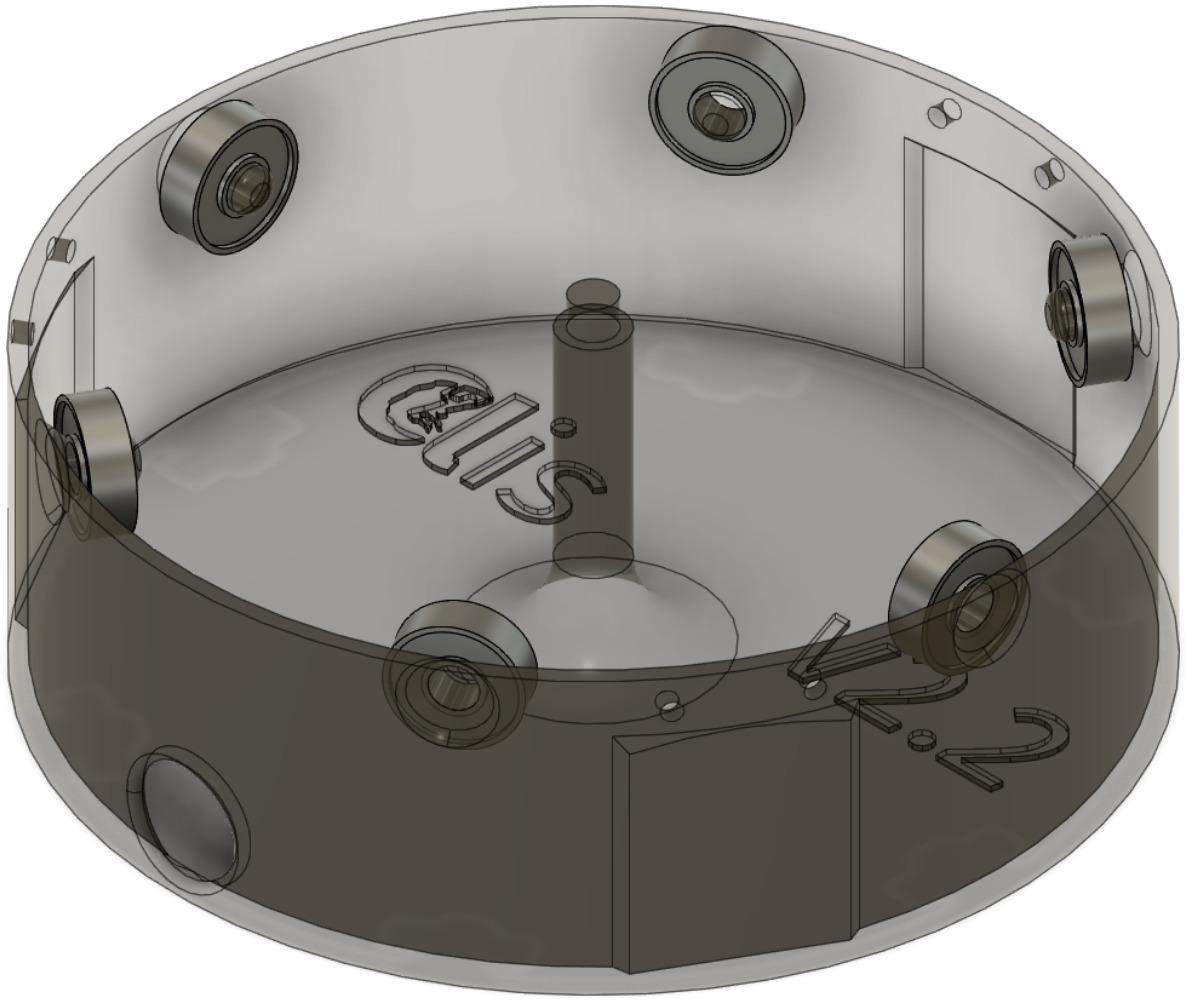
\includegraphics[height=2.2cm]{images/t1.jpg} }}% 
				\hfill
				\subfloat{{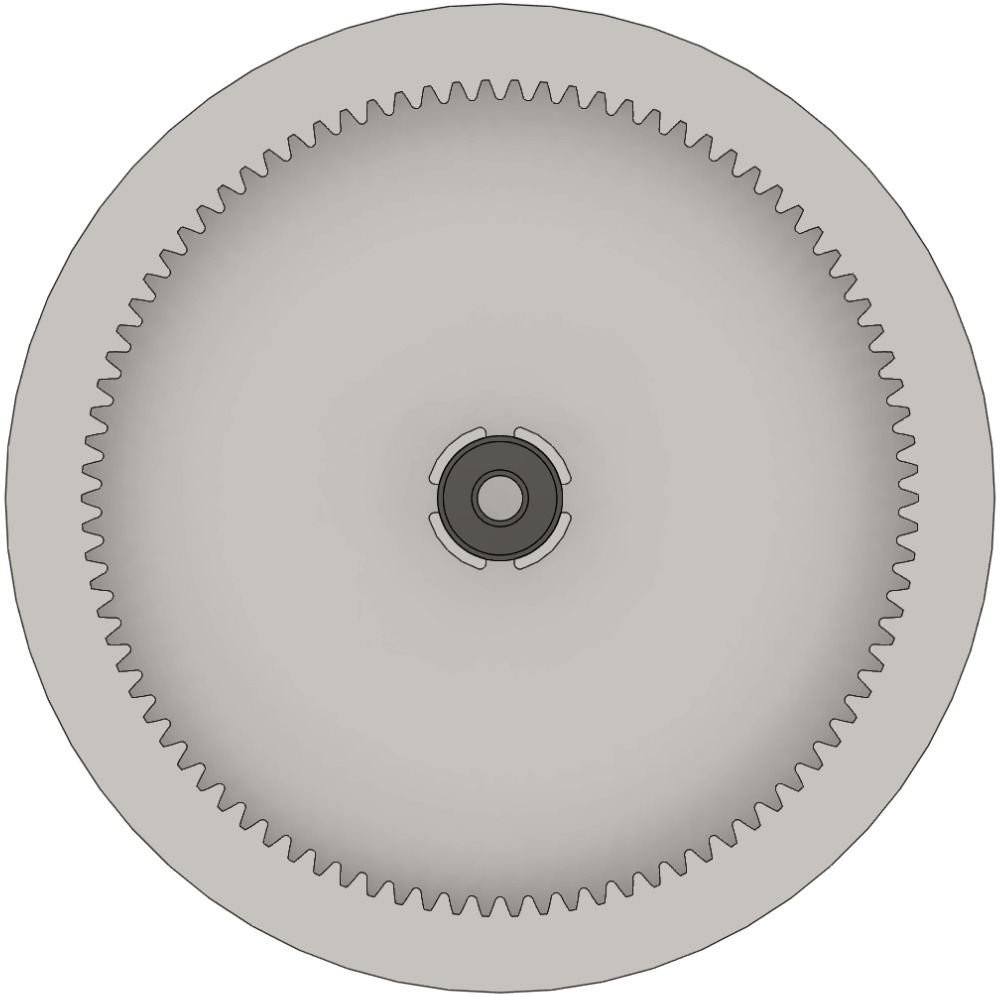
\includegraphics[height=2.2cm]{images/t3.jpg} }}% 
				\caption*{3D model otáčecího stolu}
			\end{figure}
		\end{minipage}%
		\hfill
		\begin{minipage}[t]{0.47\textwidth}
			\begin{figure}
				\centering
				\subfloat{{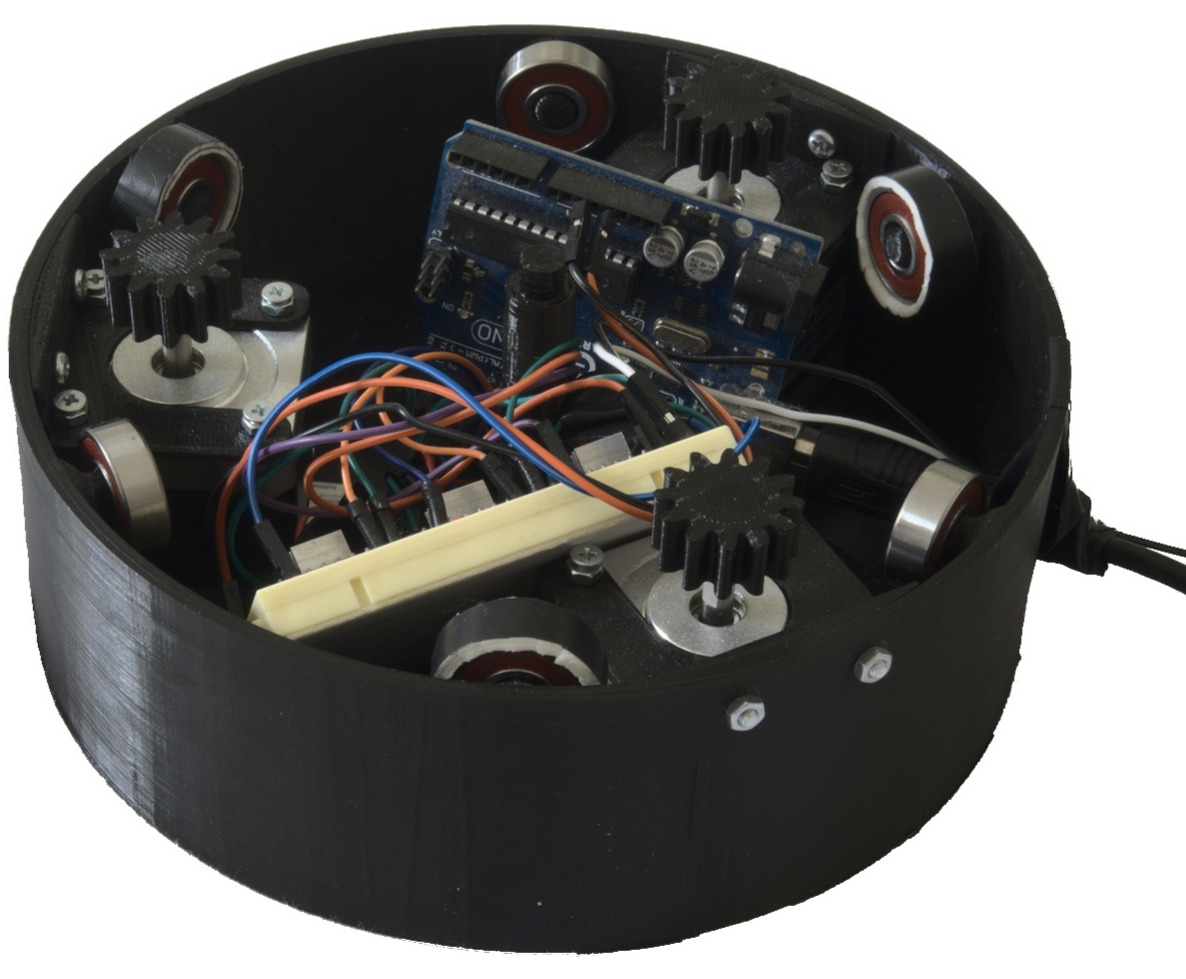
\includegraphics[height=2.2cm]{images/t4.jpg} }}% 
				\hfill
				\subfloat{{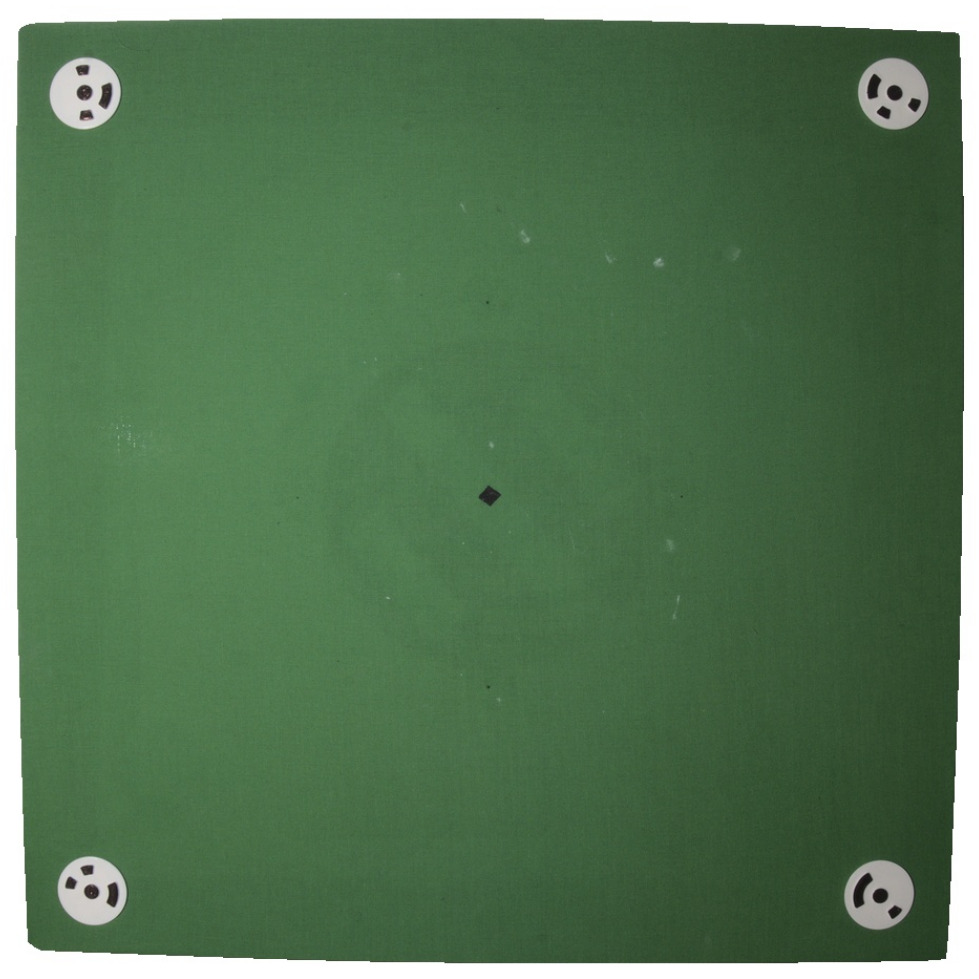
\includegraphics[height=2.2cm]{images/t5.jpg} }}% 
				\caption*{realizace otáčecího stolu}
			\end{figure}
		\end{minipage}
	\end{frame}

	\begin{frame}{Model stěny}
		\begin{enumerate}
			\item vyfocení stěny z různých úhlů (188 fotografií)
			\item vygenerování modelu přes Metashape
			\item manuální úprava v Blenderu (odstranění chyb)
		\end{enumerate}

		\vspace{0.7em}

		\begin{figure}
			\centering
			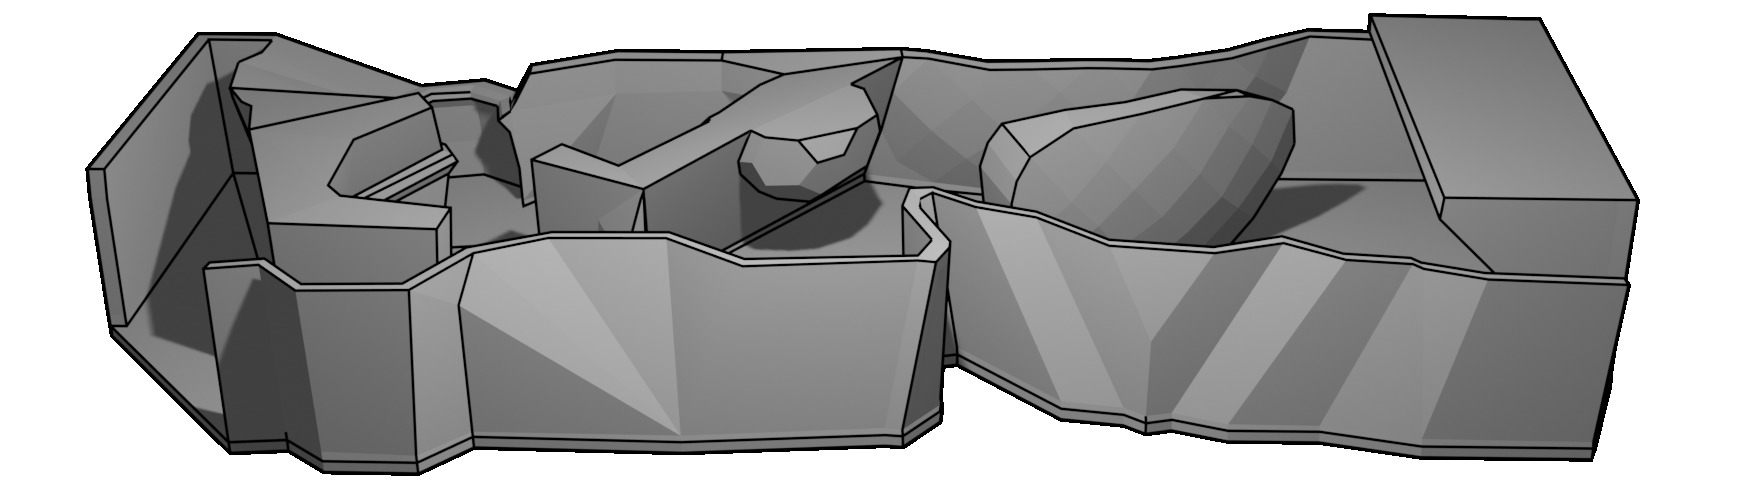
\includegraphics[height=3.0cm]{images/wall.jpg}
			\caption*{3D model Smíchoffského boulderu}
		\end{figure}
	\end{frame}

	\section{Editor}

	\begin{frame}{Přehled}
		\begin{itemize}
			\item implementace v Unity \(\rightarrow\) dostupnost na Windows a Linux
			\item GPL-3.0 licence (copyleft), sémantické verzování
			\vspace{0.7em}
			\item rozlišení módů (Normal/Holding/Route)
			\item vestavěné focení stěny z aktuální pozice kamery
			\item čitelný a parsovatelný import/export formát (\texttt{yaml})
		\end{itemize}

		\begin{minipage}[t]{0.5\textwidth}
			\fitimage[\centering výběr chytů]{images/picker.jpg}
		\end{minipage}%
		\hfill
		\begin{minipage}[t]{0.5\textwidth}
			\fitimage[\centering nastavení cesty]{images/settings.jpg}
		\end{minipage}
	\end{frame}

	\begin{frame}{Fotografie}
		\fitimage{images/capture-1}
	\end{frame}

	\begin{frame}{Fotografie}
		\fitimage{images/capture-2}
	\end{frame}

	\section{Budoucí vývoj}

	\begin{frame}{Budoucí vývoj}
		\begin{itemize}
			\item \raisebox{-0.07em}{\includesvg[height=0.8 \baselineskip]{images/clive.svg}}, the \textbf{cli}mber's \textbf{v}i\textbf{e}wer -- webový interface
			\item rozpoznávání modelů chytů z fotky a automatické umisťování
			\item laserové skenovaní pro kvalitnější modely
			\item použití VR k interaktivnějšímu stavění cest
			\item dataset pro strojové učení -- simulace lezce, st(AI)věč cest
			\item zlepšení veřejné dostupnosti: \href{https://climber.tools/}{https://climber.tools/}
		\end{itemize}

		\begin{center}
			\vspace{1em}
			\textit{Systém, do kterého se mohou zapojit stěny po celém světě.}
		\end{center}
	\end{frame}

	\begin{frame}[focus]
		Děkuji za pozornost
		\vspace{0.5em}

		\normalsize\normalfont a zejména Martinu Marešovi, Martinu Mirbauerovi, Kateřině Sulkové a Benjaminu Schillerovi za pomoc při tvorbě práce.

		\vspace{1em}

		\begin{figure}
			\centering
			\includesvg[width=0.92\linewidth]{images/climbing}
			\caption*{\href{https://xkcd.com/655/}{\color{white}{https://xkcd.com/655/}}}
		\end{figure}
	\end{frame}

\end{document}
